\documentclass[12pt]{article}

%AMS-TeX packages
\usepackage{amssymb,amsmath,amsthm} 
\usepackage{geometry, graphicx}
\usepackage{tabulary}
\usepackage{upgreek}
\usepackage{siunitx}
\usepackage{caption}
\usepackage{subcaption}
\usepackage{csvsimple}
\usepackage{enumitem}


\usepackage{pgfplotstable}
\pgfplotsset{compat=1.9}% supress warning

% setup the margins
\geometry{margin=1.0in, headheight=15pt}

\graphicspath{ {../lab03/images} }    


\begin{document}

\title{PHSX 444: Lab 03; Optical Trapping of Dielectric Particles in Liquid}
\author{William Jardee}
\maketitle

%% Introduction section. Here I introduce the physics of the experiment and give some slight motivation for the experiment. I personally think that putting the physics of the apparatus here is better. 
\section{Introduction}
The purpose of this lab was to have an introduction to particle trapping, specifically optical particle trapping. A laser, passed through a single mode fiber and culminated, was focused to a point at the end of a microscope objective. Under the objective was a solution of water and clear polyethylene microspheres, which was the target of this optical trap. These microspheres are around $1 \mu m - 1.7 mm$  in diameter, have a density very comparable to water $(0.97 g/cm^3)$ and, most importantly, are dielectric \cite{microspheres}. 

When the light hits the microspheres, the dielectric particle is attracted towards the higher electric field, from the EM wave. As it sits in this position, the rays traveling through it stabilize the height; allowing the scattering and reflected light to both push it down when it is above the balanced point, or having the scattering force pushing it down and the reflecting push it up when it is below the balancing point. The way the trap works out, in the latter case the particle is pushed back to the balancing force for small oscillations. With the planar attraction of the E-field, and the height stabilization from the reflection and scattering, particles can effectively be trapped. If this trap is thought of as a curved,  potential well, then the particle's thermal motion looks like an over-damped oscillator in that well.

The objective of this lab will be to use this method of trapping to catch these microspheres and measure their Brownian motion and mass. The Brownian motion can then be used to estimate the strength of the trap and compared against the ``escape velocity" of the trap (Figure \ref{fig:opt_trap}). Beyond these two objectives, the purpose of this lab was to become comfortable with the equipment being used, fiddling with optical devices, and use provided code to properly analyze collected data.

\begin{figure}
\centering
    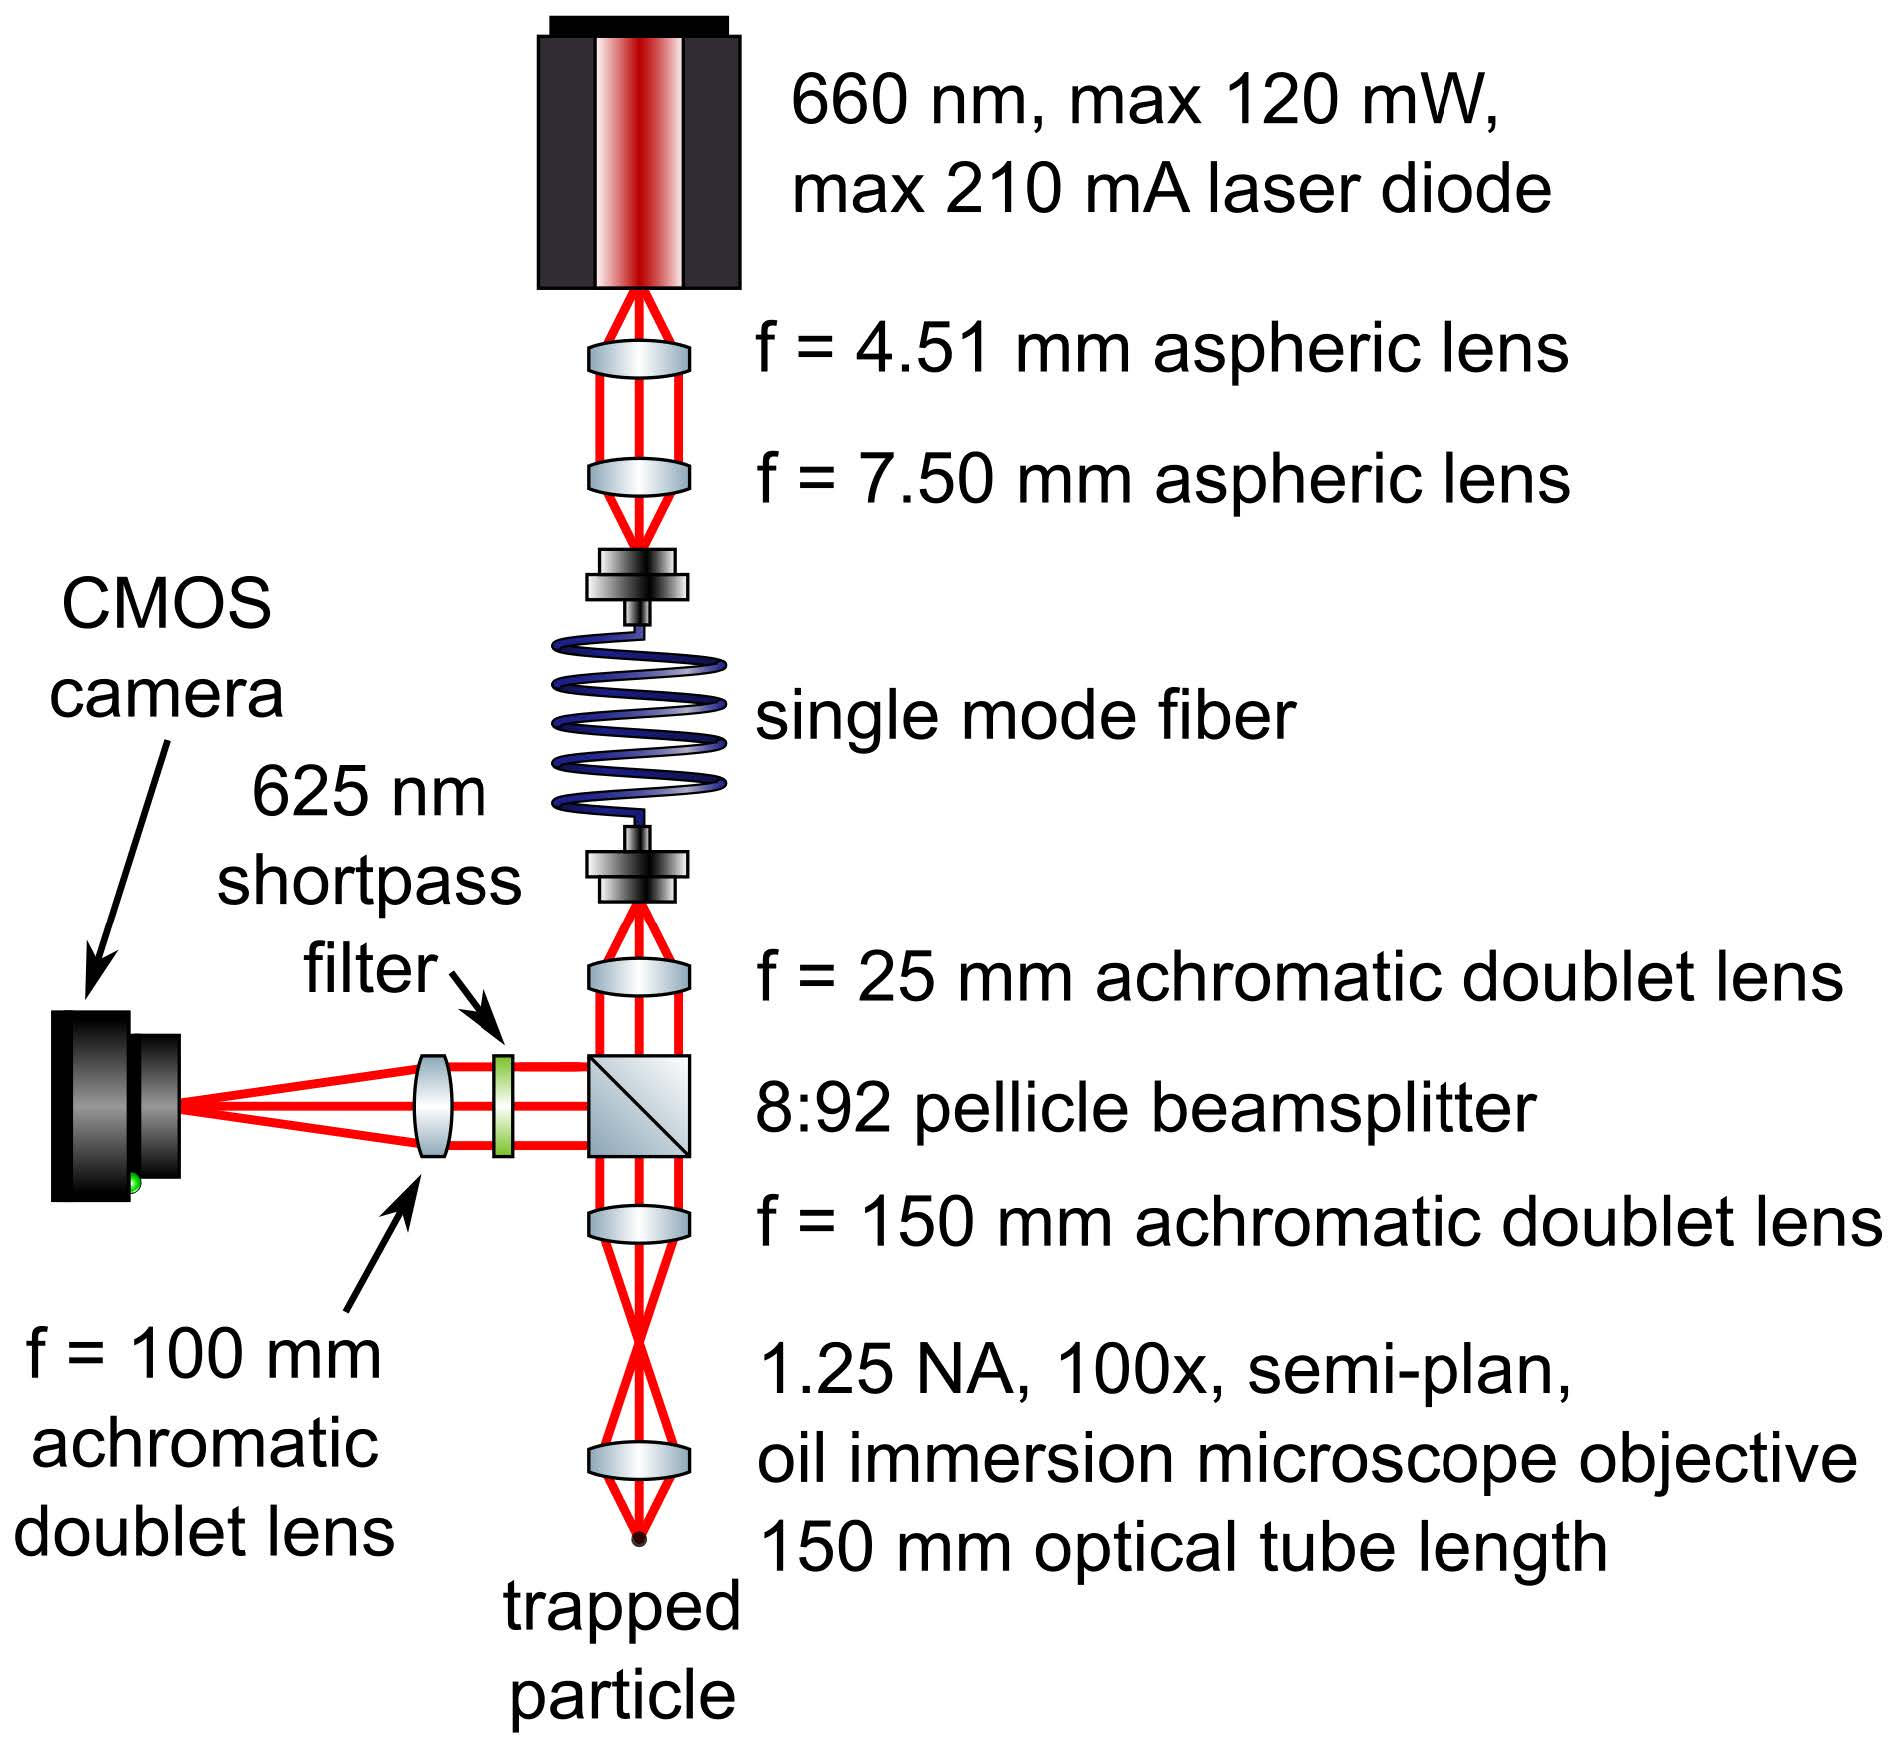
\includegraphics[width=0.5\textwidth]{optical_trap.jpg}
	\caption{Optical setup, as provided in the lab handout.}
    \label{fig:opt_trap}
\end{figure} % optical trap

The Brownian motion should represent a Boltzman distribution, where 
\begin{equation*}
P \propto e^{-E/k_B T} = e^{-(\frac{1}{2}kx^2 + \frac{1}{2}mv^2)/k_B T} \, .
\end{equation*}
Separating out the $x^2$ part and the $v^2$ part yields:
\begin{equation}
P(x^2) = A_v e^{-\frac{1}{2}kx^2 /k_B T}
\label{bolt_eq1}
\end{equation}
\begin{equation}
P(v^2) = A_x e^{-\frac{1}{2}mv^2 /k_B T}
\label{bolt_eq2}
\end{equation}
Where $x$ is the displacement from equilibrium, $v$ is the velocity, $k$ is the effective spring constant, $m$ is the particle's mass, $k_B$ is the Boltzmann constant, $T$ is the ambient temperature, and $A_v$ and $A_x$ are normalization constants.

The escape velocity allows the effective strength of the trap to measured. The force of drag on a particle in a viscous liquid is given by:
\begin{equation*}
F_\textbf{drag} = 6\pi \eta r v
\end{equation*}
where $\eta$ is the viscosity, on the order of $10^{-3} Ns/m^2$ for water, $r$ is the radius of the particle, and $v$ is the particle's speed. At the moment that the particle is able to escape, then the effective ``spring" force is equal to this drag force and the $x \approx \omega_0$, the diffraction limit of the light.
\begin{equation*}
F_\textbf{drag} = F_k = -kx \approx -k \omega_0
\end{equation*}
Putting this all together, the effective spring constant can be calculated by
\begin{equation}
k \approx \frac{6\pi r v}{10^3 \, \omega_0}
\label{eff_spring}
\end{equation}


%% Experimental Methods section. Here I go into depth about the methods used to collect the data. I also talk about where the apparatus came from. I bring up the way that we will be calibrating the data and collecting enough data to do any trend correction later 
\section{Experimental Methods}
This lab was split into three sessions; the first served to dial in the laser and collect calibration data, the second and third served to collect data. 

The first day the laser was dialed in, achieving a power output of about $3.1 \pm 0.2 mW$ from a laser diode that was current limited to $67.75 mA$. Focusing this laser into the optical setup seen in Figure~\ref{fig:opt_trap}, the calibration slide was brought into focus to calibrate the camera being used. The calibration gave a pixel size of $128 nm \times 120 nm$. This was found by taking a Fourier Transform of the calibration slide and dividing the division by the number of pixel in a period in the primary frequency peak. The orientation used in the calibration picture would be used throughout and this same calibration data will be used both days. 

The second and third sessions served as a continuing improvement on preparing slides with a plethora of microspheres on them and taking many images. Some sets of data were as simple as taking video of a particle trapped and showing a random walk. Other sets, of a much longer record period, consisted of ``playing" with the particles to experience the escape velocity, and other interactions such as adding more water to the slide and the consequential current or transferring the trapped particle to another through a forced collision.

Finally, in post the images taken were able to be cropped down only to the area of interest and processed through a given code that measured the change in position of the particle between frames. Through use of repeated correction, this code was able to get sub-pixel accuracy of a targeted position of the particle between frames . 

By using Poisson's statistics, the Boltzmann distributions in Equations \ref{bolt_eq1} and \ref{bolt_eq2} can be fit. The error at each bin's count would then be $\pm \sqrt{n}$, where $n$ is the count in that bin. This is easy enough to do with the $x^2$, as that is given by the code. Evaluating the velocity is a tad more tricky. An estimate of the average velocity between two frames will be calculated as the change in position divided by the time step between images. It will be addressed in the \textbf{Discussions and Conclusions} section whether this was a good choice.

%% Results and Analysis section. Here I go into what we actually got out of the tests and the resulting calculations from them. 
\section{Results and Analysis}

\begin{figure}
\centering
    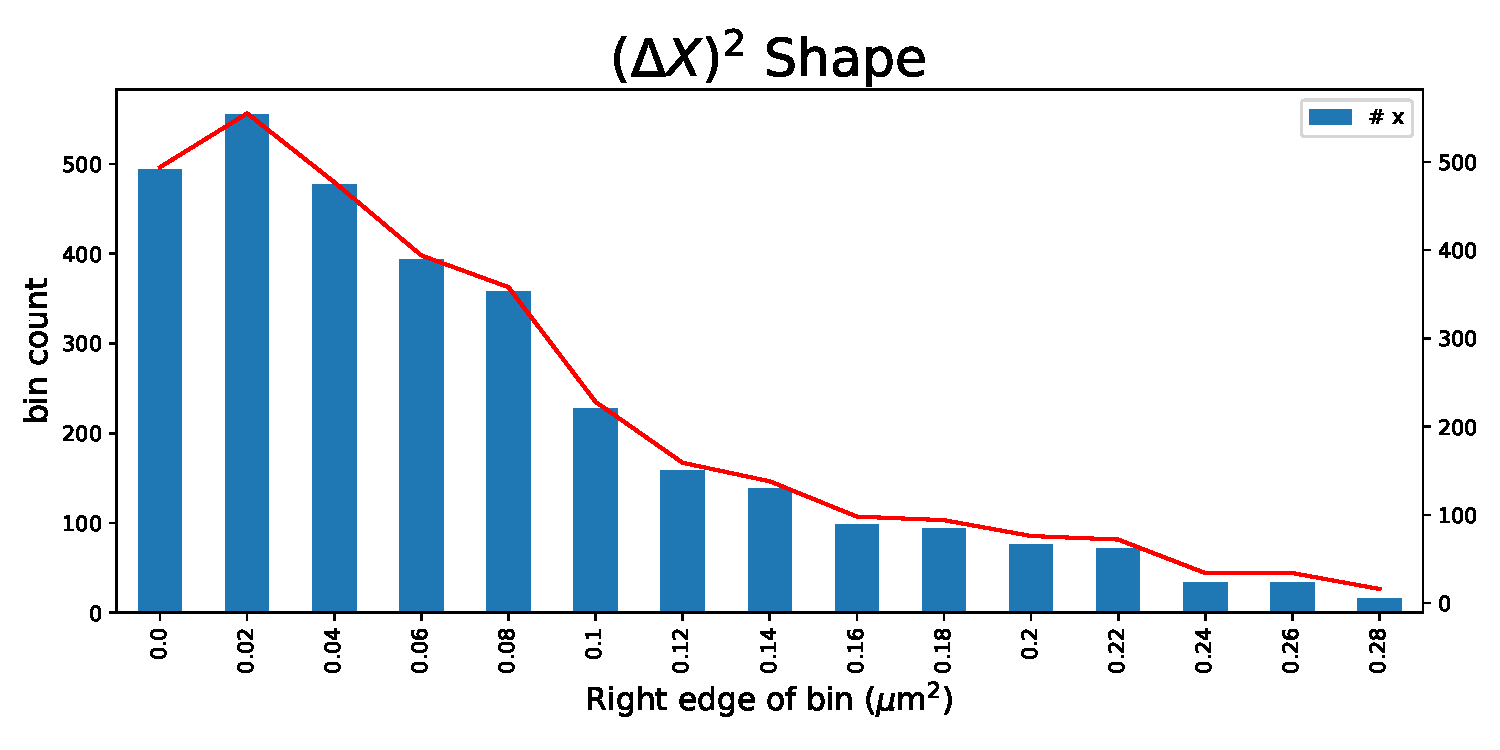
\includegraphics[scale=0.5]{primative_plot.pdf}
	\caption{The general shape of the distribution. The right edge of the bins used can be seen on the x-axis, with a bin width of $0.02 \mu m$. A red line connecting the midpoint of each bar has been superimposed on the graph to better show the Boltzmann ($e^{-x}$) distribution.}
    \label{fig:pri_plt}
\end{figure} % primative plot

\begin{figure}
\centering
    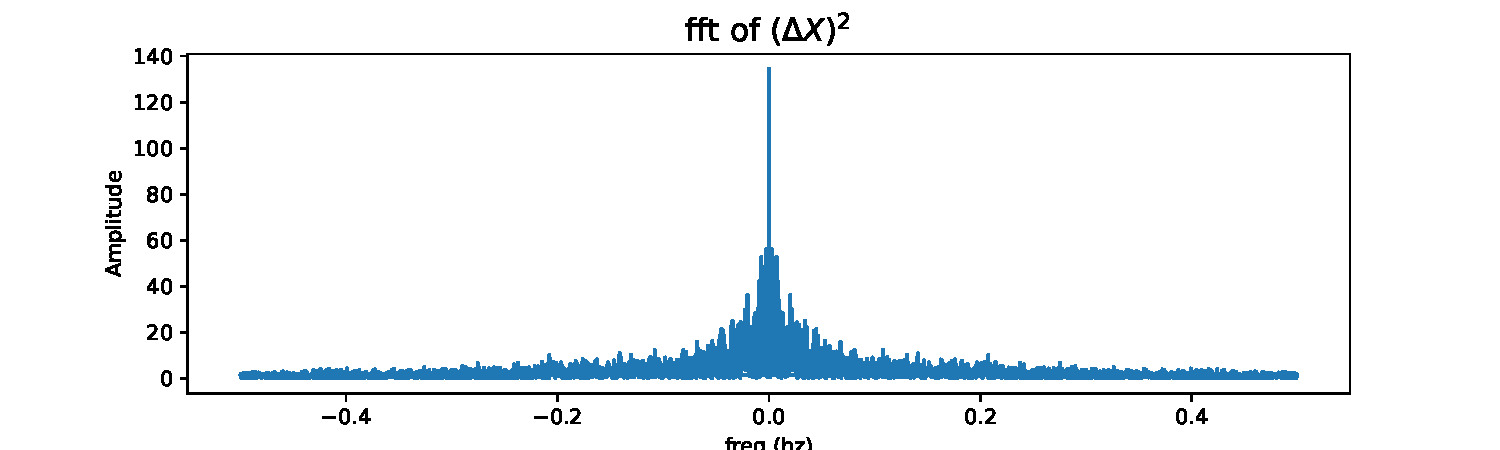
\includegraphics[width=\textwidth]{delta_x_fft.pdf}
	\caption{FFT of the $(\Delta X)^2$. This confirms the assumption that this is an overly damped system, as there is no clear peaks; in fact the curve itself seems to be an exponential decay.}
    \label{fig:delta_x_fft}
\end{figure} % delta x

\begin{figure}
\centering
    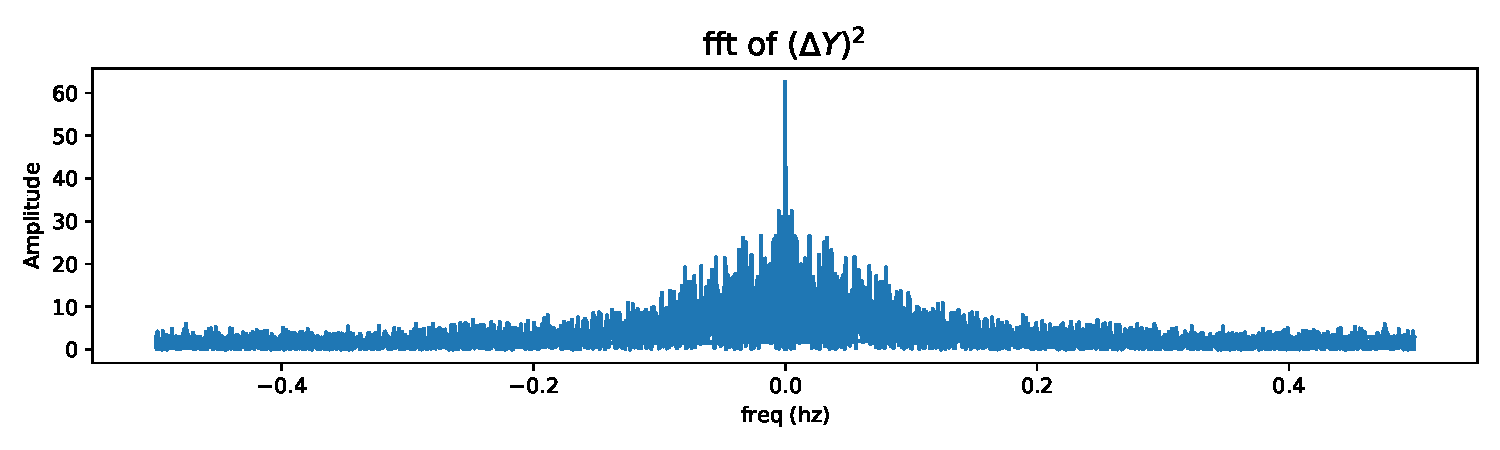
\includegraphics[width=\textwidth]{delta_y_fft.pdf}
	\caption{FFT of the $(\Delta Y)^2$ with identical characteristics as Figure \ref{fig:delta_x_fft}.}	
    \label{fig:delta_y_fft}
\end{figure} % delta y

\begin{figure}
\centering
    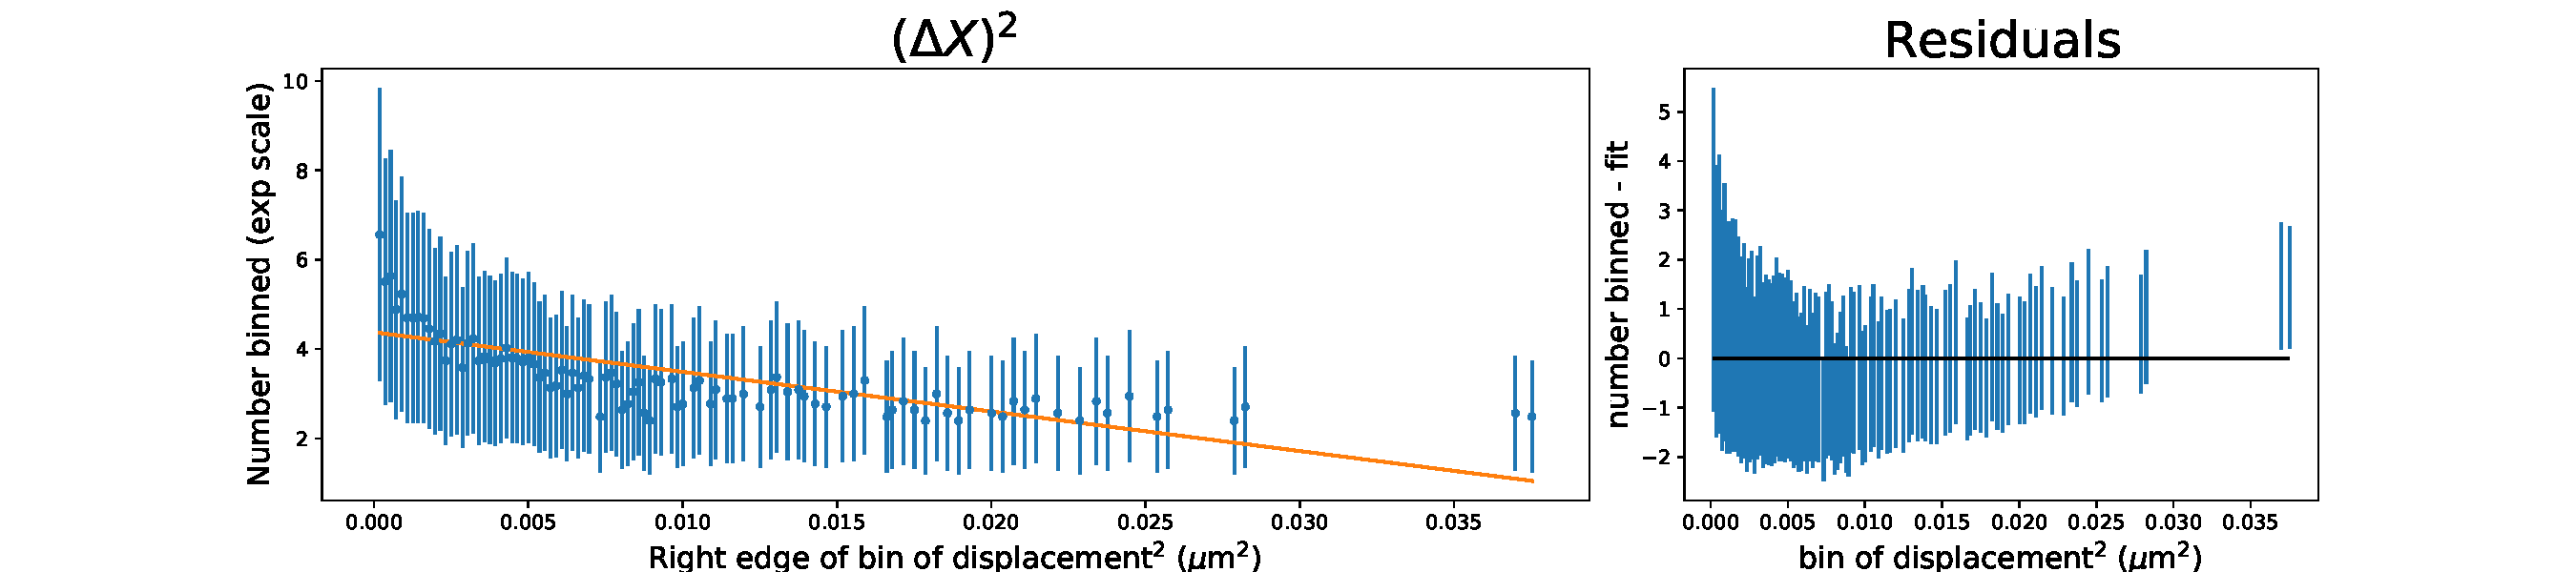
\includegraphics[width=\textwidth]{delta_x.pdf}
	\caption{The graph of displacement along the x-axis, squared. The error bars represent the error bars of the Poisson distribution ($\sqrt{n}$). The residuals can be seen to the right. Notice the quadratic artifact that seems to be left over.}
    \label{fig:delta_x}
\end{figure} % delta x

\begin{figure}
\centering
    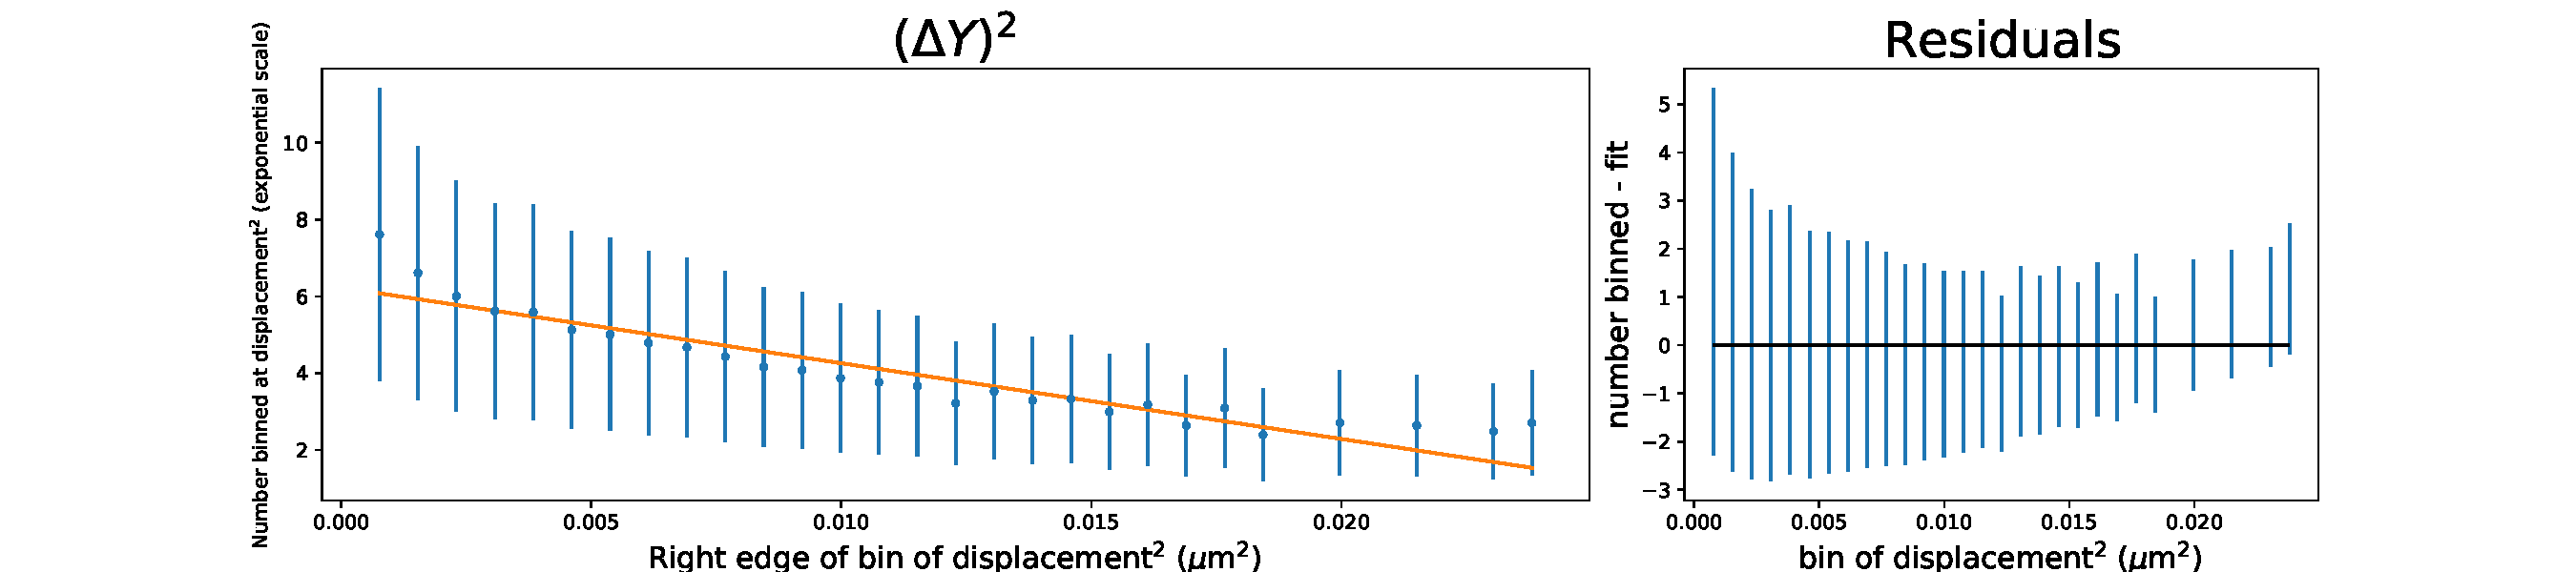
\includegraphics[width=\textwidth]{delta_y.pdf}
	\caption{The graph of displacement along the y-axis, squared. The same quadratic artifcat has been left over.}
    \label{fig:delta_y}
\end{figure} % delta y



Initially plotting the data of the square of the displacement gives some motivation for using Boltzmann statistics (Figure \ref{fig:pri_plt}). So, from here on it will be assumed that the Boltzmann statistics describe the data well. Another assumption was that this was an over-damped system. Plotting the square of the displacement in the frequency domain verified that there was no clear oscillation and that treating the system as over-damped was a valid call (Figures \ref{fig:delta_x_fft} and \ref{fig:delta_y_fft}). 

In fitting the $(\Delta X)^2$ data (Figure \ref{fig:delta_x}), the effective spring constant came out to $0.36pN/\mu m$. Fitting the $(\Delta X)^2$ data (Figure \ref{fig:delta_y}), the effective spring constant came out to $0.80pN/\mu m$. These values are compared to evaluating the strength of the trap from the escape velocity of a particle by Equation \ref{eff_spring}. The speed and $\omega_0$ can be gathered from measuring the average speed of the frames as a particle escapes from the trap. This can be done by collecting about 10 frames around the escape of the particle and choosing a stationary reference; a blemish on the slide or a stationary particle works well. Taking the pixel location of the center of the target in the first and last slide and dividing by the total elapsed time gives a good average velocity of the frames, and consequently the particle at escape. The distance between the center of the laser trap and the particle's center gives a good estimate of $\omega_0$. Collecting 5 of these escape velocities and diffraction limits gave an average escape velocity of $29.197 \mu m/s$ and average $\omega_0$ of $1.260 \mu m$. Using Equation \ref{eff_spring}, this gives $k \approx 1.12 pN / \mu m$. This is very much comparable to what was given with the other method. 


\begin{figure}
\centering
    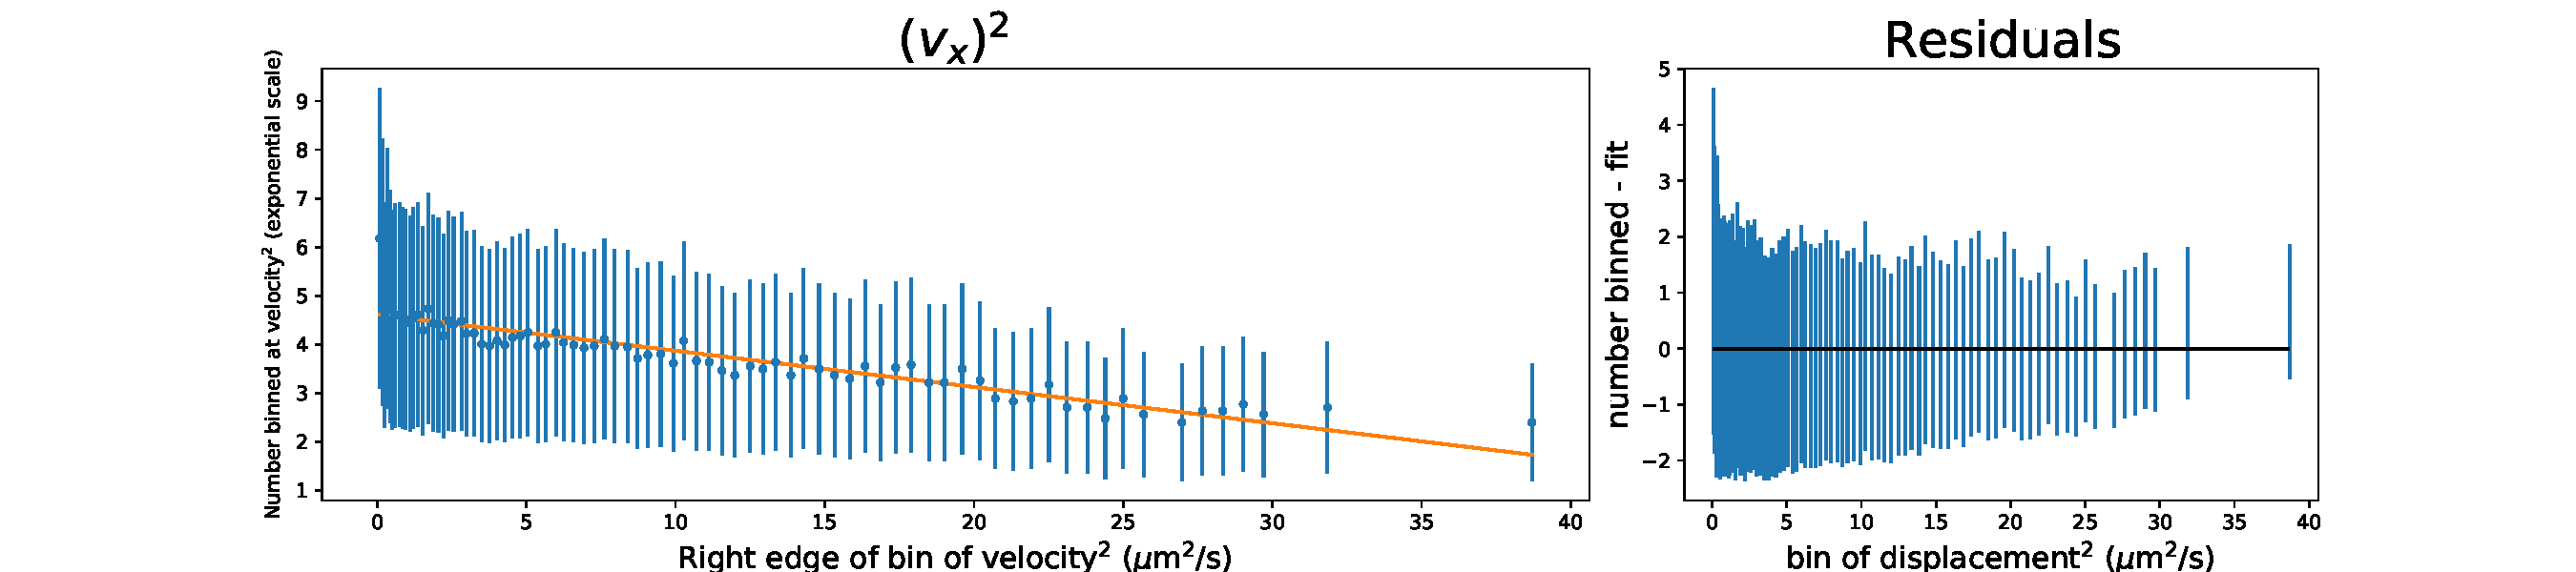
\includegraphics[width=\textwidth]{v_x.pdf}
	\caption{The fit of the squares of the velocities in the x direction calculated. This fit seems to be much better than that given in for the $(\Delta X)^2$, as seen in the residuals plot.}
    \label{fig:v_x}
\end{figure} % v_x
\begin{figure}
\centering
    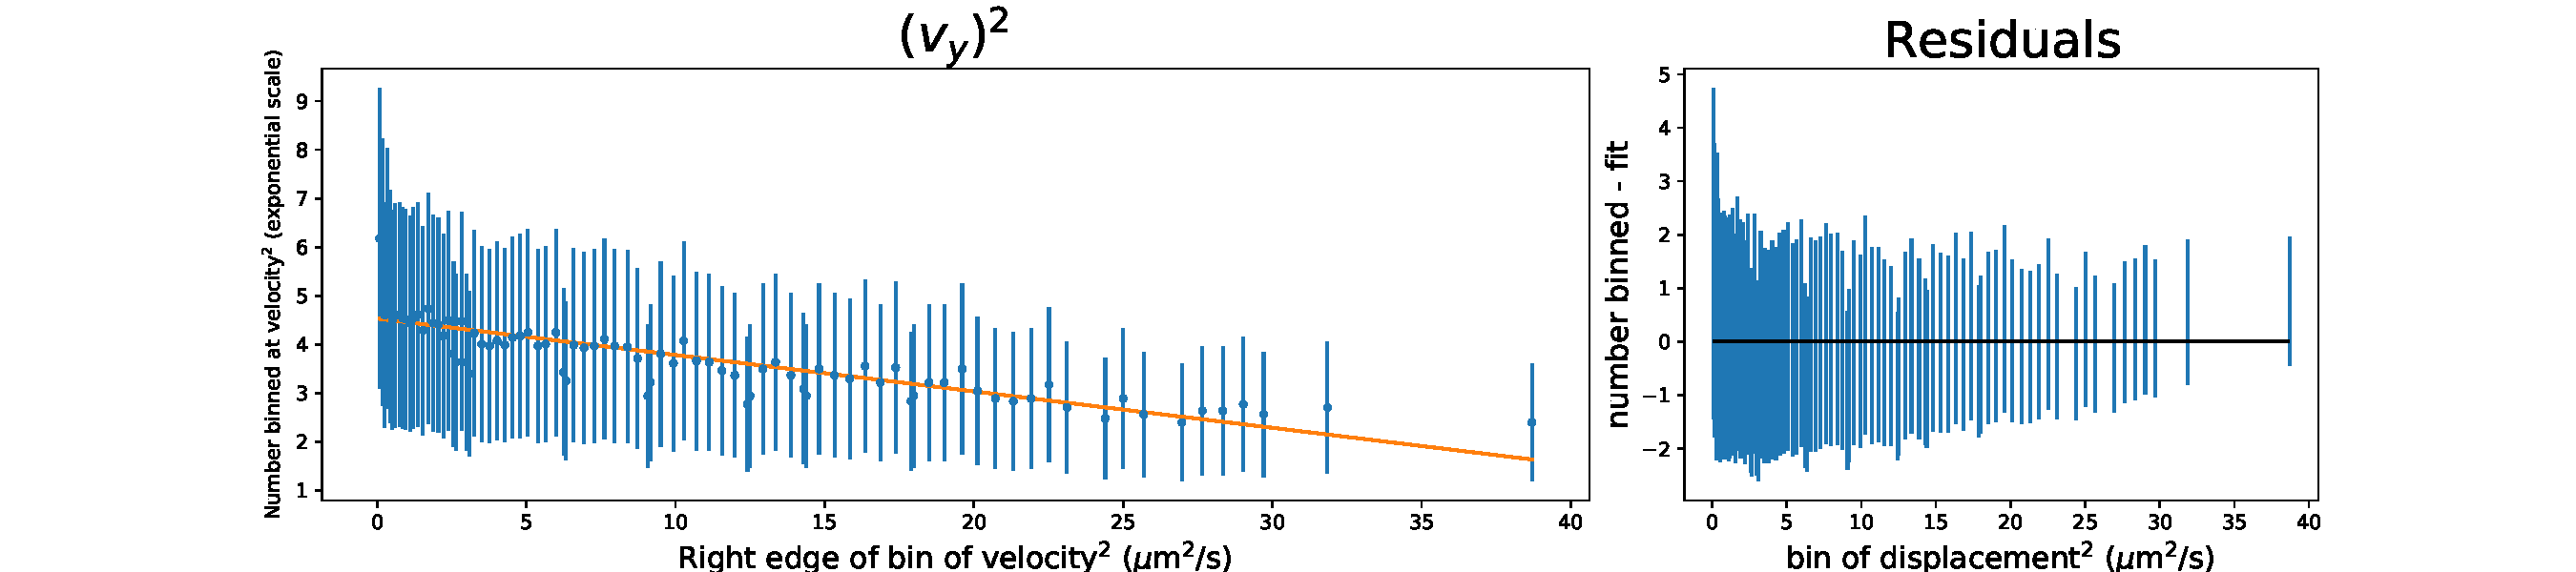
\includegraphics[width=\textwidth]{v_y.pdf}
	\caption{The fit of the squares of the velocities in the y direction.}
    \label{fig:v_y}
\end{figure} % v_y


To measure the mass of the particle, a very similar strategy was applied to the square of velocity. In fitting the $(v_x)^2$ data (Figure \ref{fig:v_x}), the effective mass came out to $0.301 \mu g$. Fitting the $(v_y)^2$ data(Figure \ref{fig:v_y}), the effective spring constant came out to $0.303 \mu g$. Analyzing both directions comes to great agreement. These values can be compared to those given by the manufacturer. Using the simple relationship of the mass of a sphere:
\[m = \rho \cdot V = \rho \cdot \frac{4 \pi}{3}r^3 \rightarrow \Big(0.97 \frac{\text{g}}{\text{cm}^3}\Big) \cdot \frac{4 \pi}{3}r^3\]\
Calculating the diameter of on of the spheres, the one used in the analysis given above, $r \approx 1.26 \mu m$. Using this value gives a mass of $m \approx 8.128 \times 10^{-6} \mu g$. This is far off from the calculated value above. If the same calculation is performed, but with a radius of $44.1 \mu m$ (35 times as large as the radius actually used), the value comes to $0.348 \mu g$. So, assuming that the method used isn't fundamentally flawed, then the effective radius of the movement of one of the particles is 35 times as large as the actual radius. This would account for the water that must be moved out of the way for the particle and end up joining this harmonic motion. 

It could be that there was some physics missed. But, it could also be a flaw in the math and/or the capturing of data. It was naively assumed that the proper way to analyze an over-damped oscillator was by used of the Boltzmann distribution. Perhaps there is another distribution that better fits this model. However, that is unlikely considering how well the same approach worked to analyze the strength of the trap. 

Another option is that the resolution in the time domain wasn't fine enough. The capture rate was about 48 fps, which comes out to about $0.02s$ per a frame. While this gives a good qualitative analysis, the way that the velocity was calculated assumes that each frame captured a straight line of movement. Instead, it is likely that between frames the particle traveled along many different vectors that averaged to the one seen. The overall speed, then, is much lower than what it should have been. A higher speed would mean that the kinetic energy is much higher, decreasing the fit parameter $m$ to account for the higher speed. The difference was 5 orders of magnitude. So, if the particle was traveling at about $10^3$ times as fast then the masses would about match. This does not take the velocity out of the realm of belief, and is reasonable for a much smaller mass. This would yield $m \approx 3 \times 10^{-7} \mu g$, which is still off by a magnitude, but much closer to the calculated value. 


\section{Discussion and Conclusions}
As seen above, the method used to trap particles, measure particle displacements, and use the data to calculate physical values have potential to be useful. The measurement of the spring constant, and in relation the strength of the trap, was very successful. However, the trap and measurement system does have downfalls. The measurement of the mass showed that in clear detail. A couple possible sources of error were also proposed; either being some missed physics or an error in the analysis of the data. All together, the experience with optically trapping such microscopic particles will be a great jumping off point for tackling more advanced traps to come. 


\bibliographystyle{unsrt}
\bibliography{references}

\begin{thebibliography}{1}


\bibitem{microspheres} “Polyethylene (PE) Precision Microspheres, Beads, Microparticles - Selection of Color, Density, Sizes 1micron to 3mm.” Cospheric, www.cospheric.com/polyethylene\_PE\_microspheres\_beads.htm. Accessed 16 Nov. 2021.

\end{thebibliography}
\end{document}
